\documentclass{article}

\usepackage{graphicx} % Required for inserting images

\usepackage{amsmath} % AMS mathematical facilities for LATEX
\usepackage{amsfonts} % TEX fonts from the American Mathematical Society
\usepackage{bbold} % A geometric sans serif blackboard bold font, for use in mathematics;

\usepackage{float} % Improved interface for floating objects

\usepackage{listings} % The package enables the user to typeset programs (programming code) within LATEX
\lstset{language=Python}
\lstset
{ %Formatting for code in Python
    basicstyle=\footnotesize,
    numbers=left,
    stepnumber=1,
    showstringspaces=false,
    tabsize=1,
    breaklines=true,
    breakatwhitespace=false,
}

\setlength{\parindent}{0pt}
\usepackage{geometry} % Flexible and complete interface to document dimensions
\usepackage{todonotes}
\geometry{hmargin=2.5cm,vmargin=2.5cm}

\title{EDIN01 Cryptography \\ Project 2}
\author{Maxime Pakula, Sofia Boselli Graf}

\begin{document}

\maketitle

\tableofcontents

\newpage


\section{Polynomials over finite fields}

\subsection{Home Exercise 1}
In this exercise the task is to determine if given polynomials are reducible, irreducible or primitive. 

\begin{enumerate}
    \item $p(x) = x^4 + x^2 + 1 \text{ over } \mathbb F_2$ \\
    As $\mathbb F_2$ only contains two elements (0,1) the amount of possible polynomials which can me multiplied to obtain the above expression is small. In this case, to obtain a polynomial of degree 4 the multiplication must be done with polynomials of degree 2 and 2 or 1 and 3. Starting with 2 and 2, there are only 4 polynomials in $\mathbb F_2$ with this constraint, and only 2 with an independent term. Calculating long division with these two yields that a reminder 0 is obtained with $x^2 + x + 1$ and:
    $$(x^2+x+1)(x^2-x+1) = (x^2+x+1)^2 = x^4 + x^2 + 1$$
    which means the polynomial $p(x)$ is reducible.
    \item $p(x) = x^3 + x + 1 \text{ over } \mathbb F_3$ \\
    In this case $\mathbb F_3$ has three elements (0,1,2). Instead of trying every possible alternative, possible roots of $p(x)$ are checked. By doing this it can be seen that $p(0) = 1$ but $p(1) = 3 = 0$ which means that there exists a way to reduce $p(x)$ with $(x-1)$ which in $\mathbb F_3$ is $(x+2)$. Calculating the results with long division the following is obtained:
    $$(x+2)(x^2+x+2) = x^3 + 3x^2 + 4x + 4 = x^3 + x + 1$$
    \item  $p(x) = x^2 + \alpha^5 x + 1 \text{ over } \mathbb F_{2^4}$ \\
    The first step is to obtain the multiplication table for $\mathbb F_{2^4}$ in order to obtain every element in the group and its expression in terms of $\alpha$ (if constructed from a primitive). If $p(x)$ is irreducible it means that $p(x) = (x-\alpha^i)(x-\alpha^j) = x^2 + (\alpha^i + \alpha^j)x + \alpha^{i+j}$. This means that for $p(x)$ to be reducible $(\alpha^i + \alpha^j) = \alpha^5$ and  $\alpha^{i+j} = \alpha^{15}$. By trying the possible alternatives a result is found with $i = 9, j=6$ which means $p(x)$ is reducible.
\end{enumerate} 

\subsection{Laboratory Exercise 1}
Now a polynomial is deemed reducible or not in Maple as follows:
\begin{enumerate}
    \item $p(x) = x^{23} + x^5 + 1 \text{ over } \mathbb F_2$ \\
    \begin{verbatim}
        Irreduc(x^23 + x^5 + 1) mod 2
    \end{verbatim}
    This returns: \textbf{True} $\rightarrow$ Irreducible
    To check if it is primitive:
    \begin{verbatim}
        Primitive(x^23 + x^5 + 1) mod 2
    \end{verbatim}
    This returns: \textbf{True} $\rightarrow$ Primitive
    \item $p(x) = x^{23} + x^6 + 1 \text{ over } \mathbb F_2$ \\
        \begin{verbatim}
        Irreduc(x^23 + x^6 + 1) mod 2
    \end{verbatim}
    This returns: \textbf{False} $\rightarrow$ Reducible
    \item $p(x) = x^{18} + x^3 + 1 \text{ over } \mathbb F_2$ \\
        \begin{verbatim}
        Irreduc(x^18 + x^3 + 1) mod 2
    \end{verbatim}
    This returns: \textbf{True} $\rightarrow$ Irreducible
    To check if it is primitive:
    \begin{verbatim}
        Primitive(x^18 + x^3 + 1) mod 2
    \end{verbatim}
    This returns: \textbf{False}
    \item $p(x) = x^8 + x^6 + 1 \text{ over } \mathbb F_7$ \\
        \begin{verbatim}
        Irreduc(x^8 + x^6 + 1) mod 7
    \end{verbatim}
    This returns: \textbf{False} $\rightarrow$ Reducible
    \item $p(x) = x^6 + \alpha^5 x + 1 \text{ over } \mathbb F_{2^4}$ \\
        \begin{verbatim}
        f := x -> x^4 + x + 1
        alias(alpha = RootOf(f(x))): Irreduc(alpha^5*x + x^2 + 1, alpha) mod 2
    \end{verbatim}
    This returns: \textbf{False} $\rightarrow$ Reducible
\end{enumerate}

\subsection{Home Exercise 2}
In this exercise the order of the following elements must be determined, this is the smallest $t$ such that $a^t = 1$. In this case from the $\mathbb F_{2^4}$ multiplicative table it is known that $\alpha^{15} = 1$ which means every element below should be taken to this number.
\begin{enumerate}
    \item $\alpha \rightarrow \alpha^t = 1 \rightarrow t = 15$
    \item $\alpha^2 \rightarrow (\alpha^2)^t = 1 \rightarrow t = 15$
    \item $\alpha^3 \rightarrow (\alpha^3)^t = 1 \rightarrow t = 5$
    \item $\alpha^5 \rightarrow (\alpha^5)^t = 1 \rightarrow t = 3$
    
\end{enumerate}
\subsection{Laboratory Exercise 2}
In this section the same task as before is done in Maple. The finite field is defined as:
\begin{verbatim}
    G218 := GF(2, 18, alpha^18 + alpha^3 + 1)
\end{verbatim}
And $\alpha$ as:
\begin{verbatim}
    a := G218:-ConvertIn(alpha)
\end{verbatim}
After this, the order of each desired element is calculated below.
\begin{enumerate}
    \item $\alpha$ \\
    \begin{verbatim}
        a := G218(alpha)
        G218:-order(a)
    \end{verbatim}
    Which returns: \textbf{189}
    \item $\alpha^2$ \\
    \begin{verbatim}
        b := G218:-`^`(a, 2)
        G218:-order(b)
    \end{verbatim}
    Which returns: \textbf{189}
    \item $\alpha^3$ \\
    \begin{verbatim}
        c := G218:-`^`(a, 3)
        G218:-order(c)
    \end{verbatim}
    Which returns: \textbf{63}
    \item $\alpha^3$ \\
    \begin{verbatim}
        d := G218:-`+`(c, a)
        G218:-order(d)
    \end{verbatim}
    Which returns: \textbf{262143}
\end{enumerate}
\subsection{Home Exercise 3}

\begin{enumerate}
    \item $p(x)=x^4+x^2+1=(x^2+x+1)^2$ \newline
    % We have the following cycle set :\newline
    % \{ \{ 0 \}, \newline
    % \{ $x \longrightarrow x^2 \longrightarrow x^3 \longrightarrow x^2+1 \longrightarrow x^3+x \longrightarrow 1$ \}, \newline
    % \{ $x+1 \longrightarrow x^2+1 \longrightarrow x^3+x^2+x+1 \longrightarrow x^2 \longrightarrow x^3+x^2 \longrightarrow 1$ \}, \newline
    % \{ $x^3+x+1 \longrightarrow x^2 \longrightarrow x^2+x \longrightarrow x^2+1 \longrightarrow x^3+x^2+1 \longrightarrow 1$ \} \} \newline
    % Note that $x^3+1$, $x^2+x+1$ and $x^3+x^2+x$ are all sent to $0$.
    To obtain the cycle set the Theorem 4.4 from the course notes can be applied. In order to do this the period of $D^2+D+1$ is calculated, as this is irreducible and primitive in $\mathbb F_{2}$ the period is calculated as $T_1 = q^L - 1 = 2^2-1 = 3$. Then $T_2 = p^mT_1$ and as $2^0<2<2^1$ then $T_2 = 2T1 = 6$. Applying all of this to the formula the cycle set is finally:
    $$1(1) \oplus 1(3) \oplus 2(6) $$

    \item $p(x)=x^3+x+1=(x+2)(x^2+x+2)$ \newline
    % We have the following cycle set :\newline
    % \{ \{ 0 \}, \newline
    % \{ $2 \longrightarrow 1$ \}, \newline
    % \{ $x^2+x \longrightarrow 1$ \}, \newline
    % \{ $2x^2 \longrightarrow 2x^2+2\longrightarrow 2x^2+x+2 \longrightarrow 1$ \}, \newline
    % \{ $x \longrightarrow x^2 \longrightarrow 2x+2 \longrightarrow 2x^2+2x \longrightarrow 2x^2+x+1 \longrightarrow x^2+2x+1 \longrightarrow 2x^2+2 \longrightarrow 1$ \}, \newline
    % \{ $x+1 \longrightarrow x^2+2x+1 \longrightarrow 2x \longrightarrow 2x^2+2x \longrightarrow x^2+1 \longrightarrow x^2 \longrightarrow x^2+2x+2 \longrightarrow 1$ \}, \newline
    % \{ $2x^2+2x+1 \longrightarrow x^2+x+2$ \}, \newline
    % \{ $x^2+2 \longrightarrow 2x+1 \longrightarrow x^2+2x \longrightarrow x^2+x+1 \longrightarrow 2x^2+1 \longrightarrow x+2 \longrightarrow 2x^2+x \longrightarrow 2x^2+2x+2$ \} \} \newline
    % Note that some cycles do not go through $1$.
    In this case $p(x)$ is the product of two irreducible functions in $\mathbb F_{3}$ which means that Theorem 4.6 in the notes can be applied. In this case $S_1 = x+2$ and $S_2 = x^2+x+2$. In the case of $S_1$ the period is calculated by long division and the result is $T_1 = 1$. This means that the cycle set for $S_1$ is simply $2(1)$. In the case of $S_2$ the function is primitive so the period is again easily calculated as $T_1 = 3^2-1 = 8$. This means the cycle set for $S_2$ is $1(1) \oplus 1(8)$. 
    Finally, the cycle set for $p(x)$ can be calculated as the defined multiplication of the cycle sets which results in:
    $$2(1) \oplus 2(8)$$
\end{enumerate}

\subsection{Laboratory Exercise 3}
Now the previous task needs to be applied in Maple. This can be done by applying every step: 
\begin{enumerate}
    \item $p(x) = x^{23} + x^5 + 1 \text{ over } \mathbb F_2$ \\
    Firstly the possibility of reducing the function is checked with:
    \begin{verbatim}
        Irreduc(x^23 + x^5 + 1) mod 2
    \end{verbatim}
    This returns true. The next step is to calculate the period, the possibility of the function being a primitive is tested:
    \begin{verbatim}
        Primitive(x^23 + x^5 + 1) mod 2
    \end{verbatim}
    Which also return true, this means that the period is calculated as:
    \begin{verbatim}
        2^23 - 1
    \end{verbatim}
    Which results in 8388607. Finally it is concluded that the cycle set is
    $$1(1) \oplus 1(8388607)$$
    
    \item $p(x) = x^{23} + x^6 + 1 \text{ over } \mathbb F_2$ \\
    Checking if reducible:
    \begin{verbatim}
        Irreduc(x^23 + x^6 + 1) mod 2
    \end{verbatim}
    yields False. The factors are obtained as:
    \begin{verbatim}
        Factor(x^23 + x^6 + 1) mod 2
    \end{verbatim}
    This concludes that: $x^{23} + x^6 + 1 = (x^{16} + x^{15} + x^{13} + x^{12} + x^8 + x^6 + x^4 + x^3 + x^2 + x + 1)(x^4 + x^3 + 1)(x^3 + x + 1)$. \\
    For $(x^4 + x^3 + 1)$ we can check that it is a primitive, the period is calculated as before and the cycle set is $1(1) \oplus 1(15)$. For $(x^3 + x + 1)$ is also primitive so the cycle set is simply $1(1) \oplus 1(7)$. 
    Finally $(x^{16} + x^{15} + x^{13} + x^{12} + x^8 + x^6 + x^4 + x^3 + x^2 + x + 1)$ turns out to not be a primitive which means the above method cannot be used to calculate the period. The algorithm to obtain the period is coded in maple in the following manner:
    \begin{verbatim}
        fun1 := x^16 + x^15 + x^13 + x^12 + x^8 + x^6 + x^4 + x^3 + x^2 + x + 1
        fun2 := 1
        
        num := 1;
        while 1 <= (tcoeff(fun2) - num*tcoeff(fun1)) mod 2 do
            num := num + 1;
        end do;
        fun2 := expand(fun2 - fun1*num*x^ldegree(fun2)) mod 2;

        while expand(fun2/x^degree(fun2)) <> 1 do 
            num := 1; 
            while 1 <= (tcoeff(fun2) - num*tcoeff(fun1)) mod 2 do
                num := num + 1; 
            end do; 
            fun2 := expand(fun2 - fun1*num*x^ldegree(fun2)) mod 2; end do;
        T := degree(fun2);
    \end{verbatim}
    After this the period obtained is T=21845. Which means the cycle set for this last polynomial is $1(1) \oplus 1(21845)$.
    Finally, to obtain the cycle set for the original equation the defined multiplication must be made, this is:
    $$[1(1) \oplus 1(15)] \times [1(1) \oplus 1(7)] \times [1(1) \oplus 1(21845)]$$. 
    Using the distributive law the following is calculated for every pair:
    \begin{verbatim}
        1*1*gcd(T2, T3)
        lcm(T2, T3)
    \end{verbatim}
    The final result is:
    $$1(1) \oplus 1(7) \oplus 1(15) \oplus 1(105) \oplus 1(21845) \oplus 1(152915) \oplus 5(65535) \oplus 5(458745)$$
    
\end{enumerate}

\subsection{Home Exercise 4}

Using an adaptation of the Sieve of Eratosthenes for the polynomials we can find the 3 irreducible polynomials of degree 4 over $\mathbb{F}_4$ :
\begin{enumerate}
    \item $x^4+x+1$
    \item $x^4+x^3+1$
    \item $x^4+x^3+x^2+x+1$
\end{enumerate}

It can be easily verified that polynomials 1 and 2 are primitive. However it can be shown that polynomial 3 is not. Let $\alpha^4+\alpha^3+\alpha^2+\alpha+1 = 0$ then $\alpha^5=1$. \newline

Therefore the two following polynomials are the only primitive polynomial of degree 4 over $\mathbb{F}_4$ :
\begin{enumerate}
    \item $x^4+x+1$
    \item $x^4+x^3+1$
\end{enumerate}

\subsection{Laboratory Exercise 4}

Using Maple we can pick random polynomials until we find one that is primitive.
\begin{verbatim}
# Create a random polynomial
a := rand() mod 5;
b := rand() mod 5;
c := rand() mod 5;
d := rand() mod 5;
f(x) := x^4+a*x^3+b*x^2+c*x^1+d;
print(f(x));

# Try if the polynomial is primitive
F16 := GF(5, 4, f(x));
alpha := F16:-ConvertIn(x);	
test := F16:-isPrimitiveElement(alpha);
\end{verbatim}

A primitive polynomial of degree 4 over $\mathbb{F}_5$ is : $x^4+3x^3+3x^2+2$

\section{De Bruijn Sequences}

\subsection{Home Exercise 5}

Using the polynomial $x^4 + x + 1$ in an LFSR and designing a special circuit to overwrite the sequence $0001 \longrightarrow 1000$ to $0001 \longrightarrow 0000 \longrightarrow 1000$ to get an FSR that has a cycle of length $2^4=16$ can be implemented in a device like the one in Figure \ref{fig:NLFSR}

\begin{figure}[H]
    \centering
    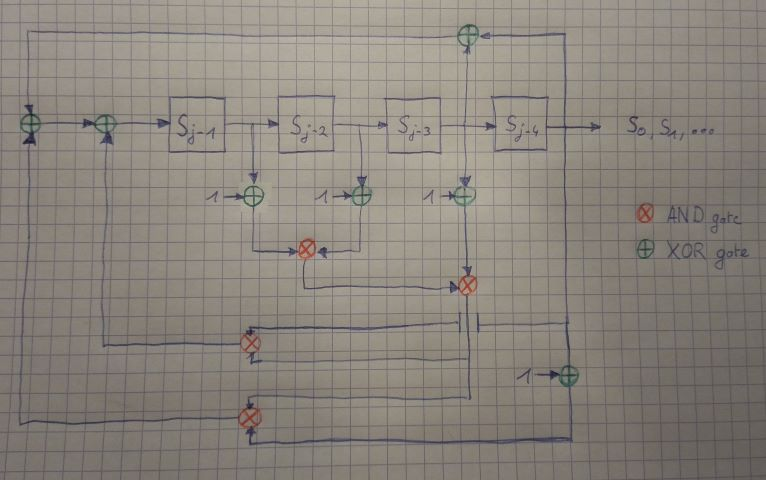
\includegraphics[scale=0.5]{NonLinearFSR.jpg}
    \caption{Non linear FSR with cycle length 16}
    \label{fig:NLFSR}
\end{figure}

\subsection{Laboratory Exercise 5}

Using the following code written in python, the desired sequence is created. The code constructs two de Bruijn sequences with cycle size $2^4$ and $5^4$ and goes through all the $10000$ different codes typing only $10003$ digits.

\begin{verbatim}
# Lab Exercise 5

def computeDeBruijn2x4(deBruijnCurrentValues_2_4) :
    # Using polynomial x^4 + x + 1

    a = deBruijnCurrentValues_2_4[0]
    b = deBruijnCurrentValues_2_4[1]
    c = deBruijnCurrentValues_2_4[2]
    d = deBruijnCurrentValues_2_4[3]

    deBruijnOutput_2_4 = d

    feedback = (d+c)%2
    if a==0 and b==0 and c==0 and d==1 :
        feedback = 0
    elif a==0 and b==0 and c==0 and d==0 :
        feedback = 1

    deBruijnCurrentValues_2_4 = (feedback,a,b,c)

    return (deBruijnOutput_2_4,deBruijnCurrentValues_2_4)

def computeDeBruijn5x4(deBruijnCurrentValues_5_4) :
    # Using polynomial x^4 + 3x^3 +3x^2 + 2

    a = deBruijnCurrentValues_5_4[0]
    b = deBruijnCurrentValues_5_4[1]
    c = deBruijnCurrentValues_5_4[2]
    d = deBruijnCurrentValues_5_4[3]

    deBruijnOutput_5_4 = d

    feedback = (2*d + 3*b + 3*a)%5
    if a==0 and b==0 and c==0 and d==1 :
        feedback = 0
    elif a==0 and b==0 and c==0 and d==0 :
        feedback = 2

    deBruijnCurrentValues_5_4 = (feedback,a,b,c)

    return (deBruijnOutput_5_4,deBruijnCurrentValues_5_4)

def computeDigit(deBruijnOutput_2_4, deBruijnOutput_5_4) :
    digit = 5*deBruijnOutput_2_4+deBruijnOutput_5_4
    return digit

def checkIfDebruijnSequence(digitsString) :
    tuplePresent = []
    for digitIndex in range(0,len(digitsString)-3) :
        currentTuple = (digitsString[digitIndex],digitsString[digitIndex+1],...
                                        ...digitsString[digitIndex+2],digitsString[digitIndex+3])
        tuplePresent.append(currentTuple)
    return len(set(tuplePresent))==10000


if __name__ == "__main__" :
    
    DE_BRUIJN_2_4_INITIAL_VALUES = (0,0,0,1)
    DE_BRUIJN_5_4_INITIAL_VALUES = (0,0,0,1)

    digitsString = ""
    deBruijnCurrentValues_2_4 = DE_BRUIJN_2_4_INITIAL_VALUES
    deBruijnCurrentValues_5_4 = DE_BRUIJN_5_4_INITIAL_VALUES

    for digitId in range(10003) :

        (deBruijnOutput_2_4,deBruijnCurrentValues_2_4) = computeDeBruijn2x4(deBruijnCurrentValues_2_4)
        (deBruijnOutput_5_4,deBruijnCurrentValues_5_4) = computeDeBruijn5x4(deBruijnCurrentValues_5_4)

        digitOutput = computeDigit(deBruijnOutput_2_4, deBruijnOutput_5_4)
        digitsString += str(digitOutput)

    file_name = "digits.txt"
    with open(file_name, 'w') as file:
        file.write(digitsString)

    isDeBruijnSequence = checkIfDebruijnSequence(digitsString)
    print(isDeBruijnSequence)
\end{verbatim}

\end{document}
